\chapter{Design}
\label{cha:Design}

This chapter discusses an overview of the proposed designs for elements required to answer the research questions. Alternative solutions are explained when relevant alongside a justification of design choices.

\section{Overall attack design}
\label{sec:attackDesign}

The attack on Trustwords involves generating "near-collision" keys. 
This attempts to provide the base to answer Research Questions \ref{goal:numberOfTrustwords} and \ref{goal:complexity}.

Near-collision keys are keys composed of a set of words that are deemed a match by the phonetic similarity metric (See Section \ref{sec:similarity_metric}). 

As each combined key in Trustwords is an exclusive-or of both sides' public-key (Equation \ref{fig:xor_trustwords} shows this process) the attack is designed to target a single pair of users and requires recomputation for every attack target. This aspect is considered when discussing the attack feasibility. Each pair is split into an "Uncontrolled" or "Controlled" key. Uncontrolled is the receiver of the communication, and, thus, the key cannot be altered. The Controlled key is the one we are attempting to impersonate. It is assumed that there is the ability to replace the Controlled key with the malicious option. These descriptions are the terminology used throughout the paper. However, the uncontrolled and controlled keys can be swapped around with the ability to compute both directions. Thus, resulting in the possibility to intercept both directions of communication. This, however, requires performing the attack separately for both directions.

\begin{equation}
    KeyFingerprint_{1} \oplus KeyFingerprint_{2} = TrustwordsFingerprint
\end{equation}
\label{fig:xor_trustwords}

When attacking a similarity metric is used to compute a list of possibilities for each position in the target fingerprint.

Figure \ref{fig:nearMatch} shows the process of generating a subsection of the combinations. A list of each words' matches is generated and combined to create the comprehensive list of near-collision keys.

\begin{figure}[h!]
    \centering
    \begin{BVerbatim}[commandchars=\\\{\}]
        \centering
\textbf{ CHOKE BLUSHING FRIGHTENING HAND}
    \end{BVerbatim}
    \\
    \verb|COKE                           |
    \\
    \verb|SMOKE                          |
    \\
    \hspace{1cm}



    \verb|CHOKE                          |
    \\
    \begin{BVerbatim}[commandchars=\\\{\}]
\textbf{COKE BLUSHING FRIGHTENING HAND}
    \end{BVerbatim}
    \\
    \verb|SMOKE                          |
    \\
    \hspace{1cm}


    \verb|CHOKE                          |
    \\
    \verb|COKE                           |
    \\
    \begin{BVerbatim}[commandchars=\\\{\}]
        \centering
\textbf{ SMOKE BLUSHING FRIGHTENING HAND}
    \end{BVerbatim}
    \caption{Visualisation of the generation of near matches}
    \label{fig:nearMatch}
\end{figure}

Completing these steps produces a list of fingerprints that can be inserted into a tool designed to hash a large number of keys and search for matches. This aspect of using a extensive list to search for keys massively reduces the complexity of the search.

In summary, the attack steps are:

\begin{enumerate}
    \item Compute all possible matches using a similarity metric on all words in a dictionary (Only needs performing once).

    \item Select a target and allocate "Uncontrolled" and "Controlled" key identification.
    
    \item Calculate all permutations of near-collisions for the key pair and produce a list of near-collision key fingerprints.
    
    \item Use a list of near-collision keys in the mass computation of keys to find near-collision keys.

\end{enumerate}

\section{Similarity metrics}
\label{sec:metrics}
One of the first requirements for the attack is quantifying "phonetic similarity." This section is looking to provide an answer for Research Question \ref{goal:phoneticSimilarity}. There are many algorithms currently available to provide this functionality. This section describes and explains the reasons they were selected for assessment later in the project.

\subsection{Soundex}
Soundex is one of the most famous example of a phonetic algorithm (See Section \ref{sec:soundex}). This is due in part to its implementation into major database clients like MySQL\cite{mysql_soundex}, Oracle\cite{moved_2005} and PostgreSQL\cite{postgresql}.

Soundex, however, has had extensive work focused on its own deficiencies alongside quantification of its performance under certain conditions. However, even with these previously discussed issues, its algorithmic simplicity and popularity allows it to remain relevant for assessment in this project.

\subsection{NYSIIS}
NYSIIS main use case was the matching of common names present in a database (See Section \ref{sec:nysiis}). However, due to it having embedded rules to handle word phonetics, it would again be applicable in this application.

Due to NYSIIS's aforementioned use in a professional setting alongside its high occurrence in literature, it was deemed suitable as one of the selected similarity metrics.

\subsection{Metaphone}
Metaphone as discussed in Section \ref{sec:metaphone} is anther famous phonetic algorithm. Metaphone is arguably on the same level of ubiquity as that of Soundex with it finding itself implemented in languages such as PHP\cite{php}. Metaphone was chosen due to similar reasons to that of Soundex and NYSIIS. 

Further work would involve the implementation of newer versions of Metaphone. Double Metaphone (2000) and
Metaphone 3 (2009) that claim to improve over the original version due to further research performed by Philips. 

\subsection{Levenshtein Distance}
As explained in Section \ref{sec:leven} Levenshtein Distance is the number of whole character edits. Levenshtein distance is not technically designed as a phonetic algorithm, but due to similar-sounding words often being spelt in similar ways\cite{hettiarachchi2012sparcl} the use-case of this algorithm remains relevant. Alongside this, Levenshtein is also the most algorithmically simplistic of all the considered options. These aspects, therefore, contribute to Levenshtein's inclusion in the chosen set.

\subsection{Phonetic Vectors}
As discussed in Section \ref{sec:phonetic_vectors} the metrics ability to perform operations and measure dissimilarity allows for a plethora of applications. One possible application of note would be the creation of a wordlist where the phonetic difference (vector distance) is maximised. This application, if the vector mapping is an accurate representation, could allow the creation of a phonetically distinctive wordlist. Therefore, these unique aspects contribute to the inclusion of this metric in the set.

\section{Alternative Similarity Metrics}

\subsection{Match Rating Approach}
Matching Rating Approach (MRA) is another algorithm designed to match names within a database; therefore, its operation can be grouped with that of NYSIIS and Soundex. MRA was discarded as an option. This removal of this metric is due to the lack of known utilisation in any substantial real-world use-cases alongside its similarity to  more established algorithms like Soundex and NYSIIS.

Further work could compare this algorithm to similar alternatives in phonetically matching of words to quantify performance. This further work is discussed in the evaluative sections of the report.

\subsection{Caverphone}
Another notable alternative solution is that of Caverphone that was designed in New Zealand. Caverphone, as is the case with the vast majority of phonetic algorithms, was designed for use with name matching. Caverphone was not chosen to similar reasons to that of MRA alongside its optimisation for the New Zealand dialect. Therefore, the low level of utilisation alongside the unique design features contributed to its exclusion. However, this has not been assessed empirically and thus would be a candidate for further work.

\begin{table}[h!]
    \centering
    \begin{tabular}{ll}
        Metric & Output \\
        \hline    
        Soundex & T614 \\
        NYSIIS & TRAVAL\\
        Metaphone & TRFL\\
        Caverphone & TRF111\\
        MRA & TRVL
    \end{tabular}
    \caption{The various phonetic encodings of the word "Travel"}
\end{table}

\section{Design of GreenOnion}
\label{sec:greenDesign}
In order to answer Research Questions \ref{goal:complexity} fully, it is necessary to implement an actual tool to generate actual keys. 

The inspiration for the design of this tool was taken from a tool called Scallion\footnote{\url{https://github.com/lachesis/scallion}}. Scallion was designed by Richard Klafter and Eric Swanson and was used to demonstrate that 32-bit PGP key IDs were insufficient. To keep with the onion-based theme, the proposed tool is called `GreenOnion' and is a re-write of Scallion in C++. This language was chosen due to the well-understood efficiency benefits. The proposed tool differs from Scallion, most notably in its ability to concurrently search for a large number of keys, GreenOnion improves on this substantially. More implementation and experimental details are discussed in later chapters.

The tool should take two keys as parameters (Uncontrolled/Controlled) and a chosen similarity metric and produce a list of target keys fingerprints. This list is then used as a search criterion when searching for keys. To utilise the parallel nature of the GPU to compute the hash of a large number of keys, the tool utilises a GPGPU (General-purpose computing on graphics processing units) framework. The chosen framework was OpenCL due to its support for the chosen language (C++) and platform (Linux). OpenCL allows the creation of code chunks referred to as "kernels" to be executed concurrently, this provides a massive speed increase compared to the sequential nature of the CPU. Technical details are explained further in Chapter \ref{cha:Implementation}.

\section{Experiment Design}
To answer some of the research questions, empirical evidence is required and, thus, experiments are required. In this section, the designs and considerations of the chosen experiments are discussed.

\subsection{Metric performance}
\label{exp:metric}
This section answers Research Question \ref{goal:phoneticSimilarity}. To reduce the number of metrics to assess in the later rounds, the performance of similarity metrics required comparison. The thinning out of metrics is required due to limited resources. Therefore, possible further work could involve repeating this work with a much more varied selection of metrics. As explained in a previous section (See Section \ref{sec:metrics}) the chosen metrics up for assessment are Soundex, Metaphone, NYSIIS, Levenshtein and Phonetic vectors.

The design for the experiment involves assessing the quality of the metrics matches by having participants rate them on a scale of 1 to 5.

\subsubsection{Matches}
\label{sec:matches}

A match for each code based metric (Soundex, Metaphone and NYSIIS) occurs when the codes are identical. However, for the other cases where the difference is variable other ways of defining a match are required.

In the case of Levenshtein values of similarity are discrete due to it being the number of single-character edits. Therefore, this requires less deliberation. Match size was used as a way to decide on a cut-off point. Match size is the number of matches determined by the metric on the English version of the Trustword dictionary (51903 unique words).

\begin{table}[h!]
    \centering
    \begin{tabular}{ll}
    Metric & Matches \\
    \hline
    Soundex     & 1,527,554 \\
    Metaphone   & 412,916 \\
    NYSIIS      & 188,474 \\
    \hline
    Levenshtein (Distance 1) [L1] & \textbf{97,730} \\
    Levenshtein (Distance 2) [L2] & 1,070,656
\end{tabular}
    \caption{Levenshtein number of matches comparison}
    \label{tab:matchSize}
\end{table}

As it can be seen from Table \ref{tab:matchSize}, the number of matches for L2 is more significant than all metrics excluding Soundex. As the issues with Soundex have been discussed in previous sections (See Section \ref{sec:soundex}) it can be excluded as an abnormality in this context. Therefore, due to the excessively high value for a L2, L1 was chosen as the Levenshtein cap for defining a match.

Match size was also used to define the threshold for the phonetic vectors. The decision is less apparent that that of Levenshtein due to the continuous nature of the distance between two vectors. However, the complexity was reduced by limiting it to increments of 0.5.

\begin{table}[h!]
    \centering
    \begin{tabular}{ll}
    Metric & Matches \\
    \hline
    Soundex     & 1,527,554 \\
    Metaphone   & 412,916 \\
    NYSIIS      & 188,474 \\
    Levenshtein & 97,730 \\
    \hline
    Phonetic Vector (Distance 3.0)  & 14,550 \\
    Phonetic Vector (Distance 4.0)  & 73,962 \\
    Phonetic Vector (Distance 4.5)  & \textbf{216,156} \\
    Phonetic Vector (Distance 5.0)  & 685,516 \\
\end{tabular}
    \caption{Phonetic vector number of matches comparison}
    \label{tab:vectorMatchSize}
\end{table}

Table \ref{tab:vectorMatchSize} contains the match size comparison for Phonetic vectors distance. Distance 4.5 was chosen as a suitable size due to the total matches fitting well within the other metrics. Distance 4.0 was the other alternative; this was discarded due to its small size. Any metric with a number of matches below 100,000 results in an inadequate number of possible near-collision keys later in the process, a lower number of matches may imply better quality, but a balance is required between computational cost and attack quality. This is discussed in more detail in later chapters.

\todo{Link the less than 100,000 point to experiment data}

\subsubsection{Comparisons}
\label{sec:exp1_comparison}
Each comparison contains a match-pair. These matches are generated by running the similarity metric over all the pairings in the Trustword dictionary, if the pair meets the criteria discussed in the previous section it is determined a match. Potential matches are then sampled from their respective lists.

Each participant is then asked to rate the similarity of a match on a scale of 1 (\textit{`Very different sound'}) and 5 (\textit{`Very similar sound'}). Figure \ref{fig:phoneticMatch} shows an example match and the connected scale. Users are provided with five of these comparisons per similarity metric.

\begin{figure}[h!]
    \centering
    \fbox{
        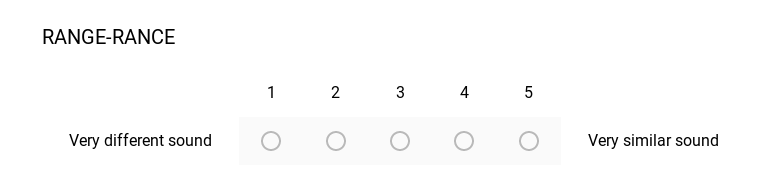
\includegraphics[width=\textwidth]{experiment/experiment_match.png}
    }
    \caption{Example experiment question}
    \label{fig:phoneticMatch}
\end{figure}

The experiment randomises the order of these comparisons per session alongside a complete refreshing of matches once per submission. This design makes sure selections from the samples are fair and consistent as each user has a different selection of matches.

\subsubsection{Quality control}
\label{sec:exp1_qualitycontrol}
As the study was being outsourced to Amazon's Mechanical Turk, the requirement to check the quality of results is essential. Therefore, a couple of additions were provided to check a result's validity.

The first was the addition of five "Random matches" questions. These are matches consisting of two random words selected from the dictionary. Therefore, the expected average rating of these words should be close to one. This design allows for a simple check for valid results. If their average is too high, their results are discarded.

\begin{figure}[h!]
    \centering
    \fbox{
        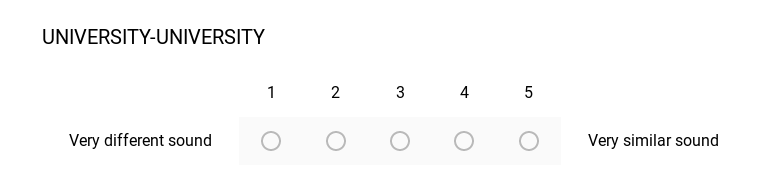
\includegraphics[width=\textwidth]{experiment/exact_experiment_match.png}
    }
    \caption{Exact experiment attention question}
    \label{fig:exactMatch}
\end{figure}

Alongside this, was the addition of two questions comparing precisely the same word. As both words are the same, the result should always be a full 5/5 rating, any results without a full rating are discarded. Figure \ref{fig:exactMatch} contains one example of the attention questions used to filter inaccurate results.

The final check to ensure the validity of results is a check for native English fluency. Having non-native English speakers complete the 
experiment can introduce inconsistencies into the 
data and, therefore, needs to remain controlled. To achieve this, a preliminary MTurk study has been created to ask users for their perceived 
English fluency on a scale of 1 (Basic Understanding) to 5 (Native). 
Workers with an answer of 5 are provided with a 
Qualification\footnote{\url{https://blog.mturk.com/tutorial-understanding-requirements-and-qualifications-99a26069fba2}} 
that tags them as defining themselves as native speakers. This qualification is then 
added as a prerequisite when running the experiment. This prerequisite ensures 
only fully native speakers are being assessed. The possibility of the 
worker falsely stating their level of fluency has also been considered. 
However, as the worker does not know the purpose of this initial study,
thereby providing inaccurate results has no real valid motive for the 
worker.

\subsubsection{Considerations}
\label{sec:exp1_considerations}

The first consideration is the way the words are compared. Due to the channel of authentication being phone-based, the comparison of words is a mixture of auditory and textual. This mixture is because a user needs to match a words sound to the one displayed on their device. This experiment asks users to compare the sound of two words that are visually displayed to them. This visual aspect is the first point of contact between the participant and the question, followed by a mental comparison of the phonetics of the word. Therefore, this initial visual contact has the potential to bias the results of the study. Levenshtein has the potential to be most affected by this due to the matches never being more than one character different, therefore, resulting in very similar-looking words. The alternative method of running this experiment is to get users to compare audio samples of words; this forces the user to compare just the phonetics of the words and not be influenced by the visual aspects of the pair. However, this adds a substantial cost to the operation of the study. Due to the aforementioned lack of resources, the chosen design was decided as most feasible as it is a balance between cost and accuracy. Further work, therefore, could improve by producing more conclusive results on the performance of the metrics by implementing the more accurate but costly alternative.

Another consideration is the demographics of people accessible on Mechanical Turk. A comprehensive and still active survey run by \textbf{D. Difallah, E. Filatova} and \textbf{P. Ipeirotis}\cite{difallah2018demographics} shows that MTurk workers are younger and have a more substantial household income than that of the US population. This deviation has to be taken into consideration when interpreting the results because it has to potential to introduce a bias.

\newpage

\subsection{Trustword Attacks}
\label{sec:exp2_design}

This experiment is designed to be a simulation of the attack proposed in Section \ref{sec:attackDesign}, in an attempt to answer Research Question \ref{goal:attackPercentage}. The experiment will test the simulated matches of three similarity metrics decided by the previous experiment (See Section \ref{sec:metrics}). The overall aim of the experiment is to quantify the success rate of the attack on live participants. The user is presented with the same design as the \pep Android application (See Section \ref{sec:pep}).

Appendix \ref{appendix:trustword_attack} shows the design of the experiments front end\footnote{A live version can also be viewed at the url: \url{https://afray.pythonanywhere.com/}}. As can be seen by comparing it to Figure \ref{fig:trustwords}, it has been designed to be as close as possible to the actual application. The blue button is clicked to simulate the authentication ceremony over the phone. A text-to-speech system then read a set of words and the user should accept if they match and decline if they don't.

\subsubsection{Design}

Due to the scarcity of attacks in a real-world setting, users are often complacent about their occurrence. Therefore, in this experiment, attacks only occur 30\% of the time. This occurrence is a much higher value than in a real-world setting, but is a balance between resources and realistic design. If the chosen attack rate is too low, many more trials are required to collate a useful number of attack instances, thus, requiring more resources but with a much more realistic design. If, however, the attack rate is too high, less total rounds are required to obtain the target number of attack trails, however, the user will lose their complacency as an attack will be expected. This loss of complacency is undesirable as it does not realistically reflect real life. Furthermore, the first 5 trials of a new experiment is always benign. This inclusion is to ensure users are consistently lulled into of complacency.

Certain keys have higher levels of potential near-collision keys than others due to how certain words are deemed similar by the similarity metric. Therefore, this presents the possibility to have keys with a very low number of possible near-collision keys. The distribution of these keys is explained further in Chapter \ref{cha:Experiments}. Therefore, if random sets of words are chosen with no restraints, there are attacks presented to the user that in a real setting would be infeasible as they are close to a $2^{64}$ attack (4 Words * 16-bits). Therefore, the experiment is designed to sample from a list of "vulnerable" keys. These are keys that have a number of potential near-collision keys that allow computation in a specified timeframe. 

Furthermore, certain levels of attacks are also simulated. Below is the list of attacks considered in this experiment: 

\begin{itemize}
    \item (\OOOO) All words in the set can vary             
    \item (\XOOO) All but the first word can vary           
    \item (\XOOX) All but the first and last word can vary  
\end{itemize}

$Where: $
\begin{itemize}
    \item[] \verb|X|: is a static word
    \item[] \verb|O|: is a changeable word
\end{itemize}

The start and ends were chosen as the highest priority words to keep static. This design choice is due to research highlighting on the common habit of users only to check the start and end of a checksum. \cite{cherubini2018towards} shows this by measuring user eye movement and displaying it as a heat map.

\begin{figure}[h!]
    \centering
    \fbox{
        \parbox{\textwidth}{
            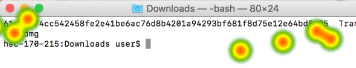
\includegraphics[width=\textwidth]{experiment/checksum_check.png}

            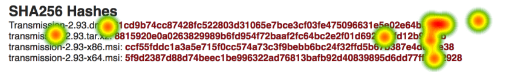
\includegraphics[width=\textwidth]{experiment/checksum_check_2.png}
        }
    }
    \caption{Failed verification of an incorrect checksum\cite{cherubini2018towards}}
    \label{fig:heatMap}
\end{figure}

Figure \ref{fig:heatMap} shows the results of an eye-tracking experiment where the user failed to detect a mismatching digest. As it can be seen, the users never compared the centre of the digest. 

However, this may not be applicable in this context due to the user being linearly fed an audio stream that they cannot skip to the start or end. We believe, however, that attention also plays a part in defining the most important areas of comparison. The hypothesis is that the users' attention is lower in the middle sections of comparison, where it peaks at the start and end. All of these aspects require empirical evidence to conclude. Therefore, this requires consideration when assessing the results of the experiment.

These attacks are ascending in complexity. The timeframe for computing a near-collision was decided as 7-days with attack strengths of 1 GPU-day, 10 GPU-days and 100 GPU-days on a mid-range GPU (AMD RX 480). Due to the long lifetime of PGP keys, 7 days was chosen as a reasonable length of the attack. The tool requires no user interaction once started, therefore, it can be left for an extended period to compute potential keys. This timeframe is also a maximum time, these attacks also include keys that have a shorter average computation time.

\begin{table}[h!]
    \centering
    \begin{tabular}{lll}
    GPU/days & No of combinations required & Attack Type \\
    \hline
    1       & 15250   & Zero static\\
    10      & 1525    & One static\\
    100     & 152     & Two static\\        
\end{tabular}
    \caption{Summary of attack requirements}
    \label{tab:attackReq}
\end{table}

Table \ref{tab:attackReq} contains a summary of the different level of attacks and their respective restrictions. More potential near-collision keys make the attack search quicker. Any key that exceeds the defined numbers of potential near-collision key for attack level are deemed as vulnerable.  As discussed in Section \ref{sec:attackDesign} the near-collision keys are close keys produced from the similarity-metric's matches. A list of these vulnerable keys is sampled from when an attack is simulated. The percentage of vulnerable keys is explored in Chapter \ref{cha:Experiments}.

\subsubsection{Quality control}
\label{sec:exp2_quality}
Like the previous experiment, participants are sourced from MTurk. Therefore, again, quality control is an aspect that requires consideration. As with the previous study, initially screened native speakers are used, alongside the utilisation of the same process to recruit suitable workers. Two metrics are used to detect invalid results: audio-button-clicks and the overall-time. 

Audio-buttons-clicks is the number of times the blue \textit{"Authenticate with partner over the phone"} button in Figure \ref{fig:expID} is clicked. If there are rounds without button clicks, this is a sign of non-attentiveness. The design choice was made to keep this as a result filter, as preventing non-clicks would be a trivial task. This design provides a way to detect and discard click-throughs\footnote{Workers that aim to complete the task as fast as possible, with no regard for the quality of responses}. 

Overall-time is as the name suggest a recording of the time taken to complete the entire experiment. If users complete the experiment in an abnormally small amount of time, it can be used as another detection for invalid responses. A benchmark for the time is set by completing the experiment correctly but as fast as possible. Anything below this pace was discarded as anything higher will risk invalid and rushed results.

\subsubsection{Considerations}
As with the previous experiment, sampling from a  MTurk demographics results in a collection of participants that are not reflective of the general population. Due to the attack context of this experiment is can be assumed that the youth of the participants contributes to less successful attacks. Therefore, the results generated by this experiment can be loosely assumed as a best-case scenario for the scheme. We predict a high attack success rate if assessed over the general population.